\section{Internal Voltage Model (ivmmod)}  
The \verb|ivmmod| model was created by Dr. Trudnowski to simulate a voltage-behind an impedance generator in PST.
The new `internal voltage model' is meant to mimic the actions of a grid-forming inverter based generator.
Figure \ref{fig: ivmmod BD} shows how a generators internal voltage $E_i$ and angle $\delta_i$ may be manipulated by a user created function \verb|ivmmod_dyn.m|.
Any number of model structures can be modeled is the user supplied controls model.

\begin{figure}[H]
	\centering
	\footnotesize
	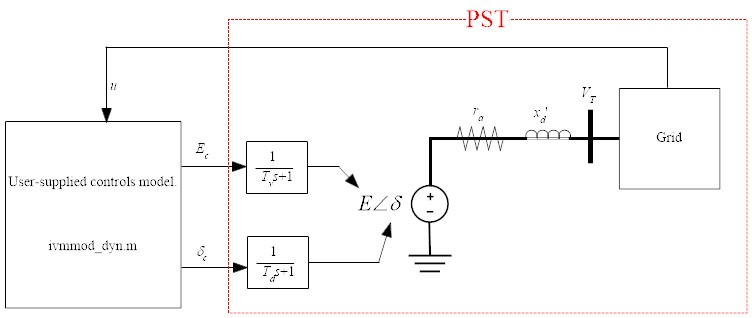
\includegraphics[width=\linewidth]{sections/ivmmod/IVM_Model}
	\caption{Block diagram of internal voltage model.}
	\label{fig: ivmmod BD}
\end{figure}%\vspace{-1 em}

To define an \verb|ivmmod| generator, the desired bus must be set to type 2 in the \verb|bus| array, and a row in the  \verb|mac_con| array is used to define set parameters of the model.
Listing \ref{lst: ivm example} provides an example of a \verb|mac_con| \verb|ivmmod| definition.
The model is recognized in PST by setting the inertia constant $H$ (column  16) to zero.

\pagebreak
\begin{lstlisting}[caption={IVMMOD Definition Example},label={lst: ivm example}]
\end{lstlisting}\vspace{-2 em}
\begin{minted}[
		frame=lines,
		framesep=2mm,
		baselinestretch=1.2,
		bgcolor=gray!13,
		fontsize=\footnotesize,
	%	linenos,
		breaklines
				]{MATLAB}
%% IVM definition format:
% col 1       generator number
% col 2       bus number
% col 3       generator MVA base
% col 4       Not used
% col 5       r_a
% col 6       Not used
% col 7       x’_d
% col 8       Not used
% col 9       Td
% col 10      Tv
% col 11      Not used
% col 12      Not used
% col 13      Not used
% col 14      Not used
% col 15      Not used
% col 16      0 (this is H for a syn generator)
% col 17      Not used
% col 18      Not used
% col 19      bus number

% An example:
mac_con = […
% 1   2   3    4  5   6  7    8  9    10   11 12 13 14 15 16 17 18 19
% num bus base NA r_a NA x'_d NA Td   Tv   NA NA NA NA NA 0  NA NA bus
   3   2  100  0  0   0  0.1  0  0.05 0.05 0  0  0  0  0  0  0  0  2];
\end{minted}

An example of the \verb|ivmmod| is presented in Section \ref{sec: ivmmod ex}.
Currently, the \verb|ivmmod| is only available in non-linear simulation.


%While there are questions about the reality of such operations and how PST simulates them, the model exists and appears to `work' in the non-linear simulation  of PST 4.
